% !TeX spellcheck = en_GB
\section{Question 3}

\subsection{A)}
\begin{quote}
	\textit{"Assume	that	the	data	from	project	3	is	not	a	massive	data	set,	but	a	data	stream.	Every	time	step,	a	large	collection	of	vehicles	and	persons	is	generated	(based	on	the	attributes	contained	in	the	<vehicle>	and	<person>	elements	of	the	XML	file	given	in	project	3).	How	would	you	proceed	to	characterize	such	a	data	stream?"}
\end{quote}
The data of the stream contains structured data since it is in XML format. The structure is as follows:
\begin{verbatim}
<Timestep>
    <vehicle, id, x, y, angle, type, speed, pos, lane, slope/>
</Timestep>
\end{verbatim}
or 
\begin{verbatim}
<Timestep>
    <person, id, x, y, angle, speed, pos, edge/>
</Timestep>
\end{verbatim}
depending on which type the input has. This information, since it is in XML is easily obtained since the structure of the data is part of the data itself. Had the data been in JSON format it would be more difficult, albeit not impossible to find this structure, and had the data been unstructured it would have been even more difficult, since one should try to create and fit a schema at the same time.

Furthermore to describe the data stream one could examine the number of discrete elements that are present over timesteps in total or an average of that. Given these values it becomes obvious that we need big data systems to handle the stream. This could be done either with batch jobs, but it could also be done by making windowed stream analysis. By examining a window in the stream one could approximate the average amount of entities pr timesteps. 

\subsection{B)}
\begin{quote}
		\textit{"Describe	a	meaningful	view	based	on	the	data	set	from	the	Project	2	data	set.	How	do	you	obtain	that	view?	Describe	the	problems	you	faced	obtaining	such	views	in	project	2	and	how	you	fixed	them."}
\end{quote}
I have chosen to showcase the second view from our Project 2 as I find that the most interesting. The view was described as follows: 
\begin{quote}
	\textit{"How can Wi-Fi data be used for tracking an individual at ITU?"}
\end{quote}
The hypothesis is that information about what access points a client has been connected to makes it possible to track a single person at ITU. Since each Wi-Fi client has an unique ID in the data set, tracking that ID around the ITU through various access points in certain rooms, one could connect this information to teaching activities. One could essentially build a schedule corresponding to a person, the holder of the unique ID, and by cross referencing the public course base, identify any student or teacher. 


It is necessary to assume that every person is connected to Wi-Fi whenever they are at ITU and even more important that they are connected to the access points in the rooms that they have courses in. 

To obtain the data we created a map-reduce program. The main part of the analysis is done in a mapper. The map method can be seen in figure \ref{code:project2_mapper}. The method tests the entity for null values, and whether its a WiFi client or an accespoint. Then the entity is correlated to a specific access point. Going over all the information of that access point at that time. 

 \begin{lstlisting}[frame=single, backgroundcolor=\color{light-gray}, basicstyle=\footnotesize\ttfamily, language=Java, numbers=left, numberstyle=\tiny \color{black}, breaklines=true, label=code:project2_mapper]
 
public void map(AvroKey<Readings> key, NullWritable value, Context context) throws IOException, InterruptedException {
    Readings readings = key.datum();
    if(wifiMap.containsKey(readings.getUUID().toString()))
	{
        WifiClient wifiClient = wifiMap.get(readings.getUUID().toString());
		if(wifiClient.getTypeOfMeasure().equals(WifiClientMeasure.AccessPoint))
		{
		    for(Reading reading : readings.getReadings())
			{
				AccessPoint ap = apMap.get(reading.getValue());
				if(ap != null && ap.getLocationId() != null && locationMap.containsKey(ap.getLocationId()))
				{
					Date date = new Date(reading.getTimeStamp());
					Location location = locationMap.get(ap.getLocationId());
					 
					context.write(new Text(readings.getUUID().toString()), new Text(location.getRoom() + "-" + dateFormat.format(date)));
				}
			}
		}
	}
}
\end{lstlisting}

It becomes obvious that having this as one mapper does use the map-reduce framework to its full potential. It would have been a better idea to split this into multiple mappers, for example in the situation where the mapper iterates over the readings, it would have been smarter to use a mapper for that job. This could greatly increase the parallization and therefore the scalability of the batch job.

The reducer simply aggregates the rooms, times together to a list over each specific wificlient.

A snippet of the output can be seen in figure \ref{fig:result_data}
\begin{figure}[p]
	\caption{Resulting data}
	\label{fig:result_data}
	\begin{verbatim}
	...
	fd958189-5ad3-5586-a7ad-d3fe4e6f4695	
	    4A32-2016-10-12:11, AUD44A60-2016-10-24:08, AUD44A60-2016-10-24:09, 
	    AUD32-3A56-2016-10-04:09, AUD32-3A56-2016-10-04:08, 5A60-2016-10-12:07, 
	    4A58-2016-10-24:08, AUD44A60-2016-10-10:09, AUD32-3A56-2016-10-04:10, 
	    3A12-2016-10-06:11, 3A12-2016-10-06:12, 5A07-2016-10-12:11, 
	    AUD32-3A56-2016-10-13:09, 5A05-2016-10-31:11, 5A07-2016-10-12:10,
	    3A52-2016-10-25:11, 3A52-2016-10-25:10, AUD44A60-2016-10-24:10,
	    4A58-2016-10-24:09, AUD44A60-2016-10-31:10, 4A16-2016-10-24:14,
	    5A07-2016-10-05:08, 4A16-2016-10-24:11, 4A16-2016-10-24:13,
	    4A16-2016-10-24:12, 5A07-2016-10-12:08, 5A07-2016-10-12:07,
	    AUD32-3A56-2016-10-25:10, AUD44A60-2016-10-10:10, 4A58-2016-10-24:10,
	    5A07-2016-10-12:09, 4A16-2016-10-10:12, 4A16-2016-10-10:11,
	    4A16-2016-10-10:14, 4A16-2016-10-10:13, 4A22-2016-10-31:13,
	    4A05-2016-10-12:11, AUD32-3A56-2016-10-06:09, AUD32-3A56-2016-10-13:10,
	    5A07-2016-10-05:09, AUD32-3A56-2016-10-25:09,
	...
	\end{verbatim}
\end{figure}

Which can be represented a bit better visually in a schema as seen in figure \ref{fig:result_schema}.

\begin{figure}[p]
	\centering
	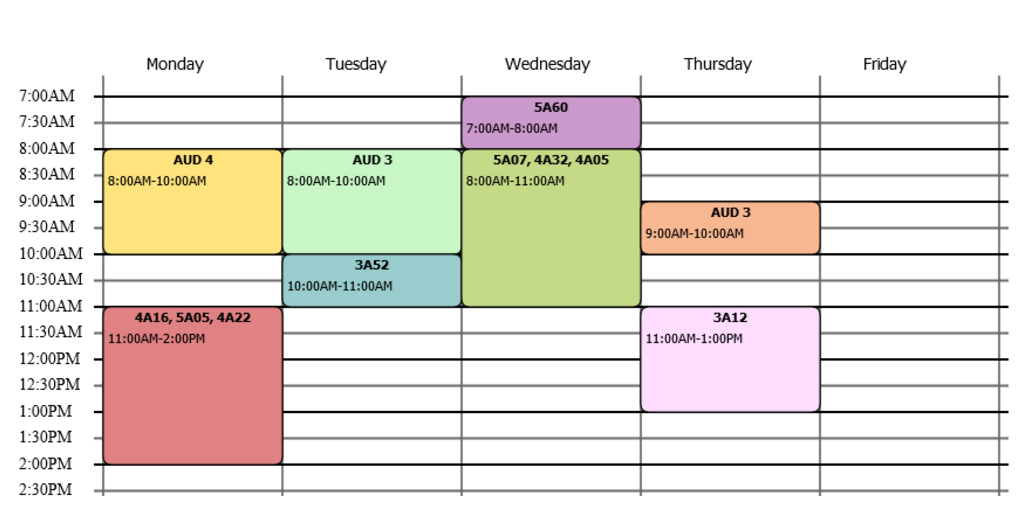
\includegraphics[width=\linewidth]{figures/schema-from-data.png}
	\caption{Resulting Schema}
	\label{fig:result_schema}
\end{figure}

With these results, we can put together a schema for the person and match it with course information and TimeEdit, to find the rooms the person have been around. The most plausible result is, that it is a 1st year GBI student, since the schemas match.

\begin{figure}[p]
	\centering
	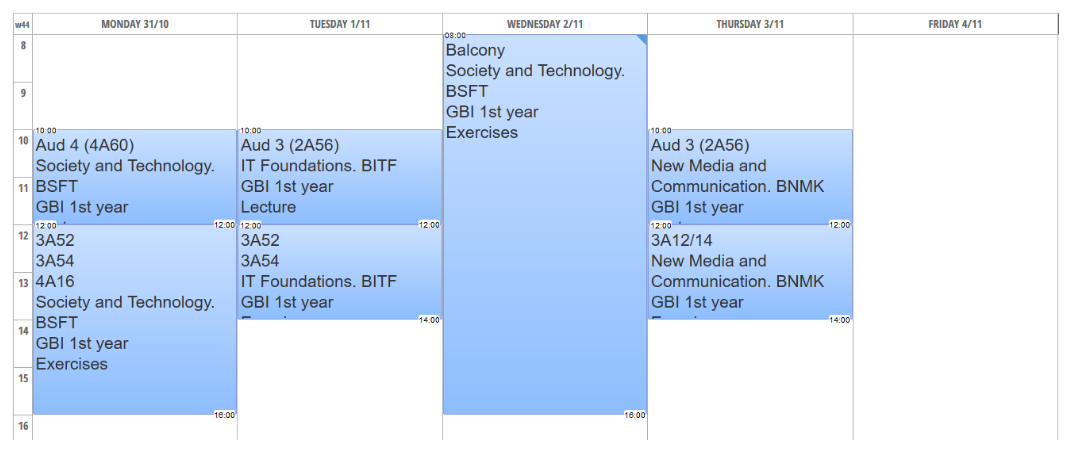
\includegraphics[width=\linewidth]{figures/schema-from-timeedit.png}
	\caption{Timeedit Schema for a 1st year GBI student}
	\label{fig:timeedit_schema}
\end{figure}

One of the most difficult parts of creating this batch view was handling the difference between WiFi clients and Access Points. 
